\documentclass[10pt,a4paper]{article}
\usepackage[utf8]{inputenc}
\usepackage{amsmath}
\usepackage{amsfonts}
\usepackage{wrapfig}
\usepackage{amssymb}
\usepackage{enumitem}
\usepackage{graphicx}
\usepackage{lipsum}
\graphicspath{ {images/} }
\author{Martina Salvati}
\title{ANALISI CONSUMI ENERGETICI TRAMITE POWERAPI}
\date{\today} % Sets date for date compiled
\begin{document}
\maketitle
\listoffigures

\begin{figure}[h]
\caption{CONSUMI ENERGETICI GLOBALI}
\centering
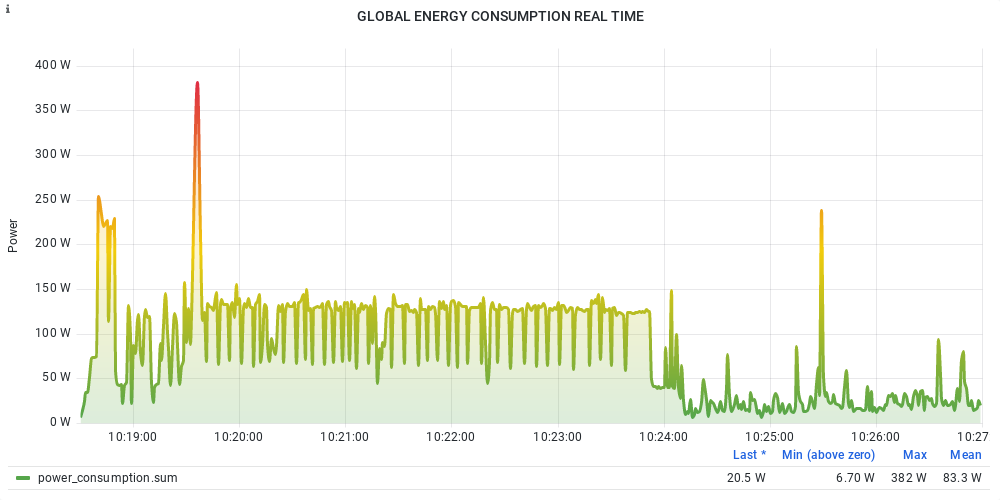
\includegraphics[scale=0.4]{image2}
\begin{flushleft}
{Per la rappresentazione di questo grafico viene fatta la somma ogni secondo della potenza istantanea}
\end{flushleft}
\end{figure}
\begin{figure}[h]
\caption{ENERGIA MEDIA CONSUMATA}
\centering
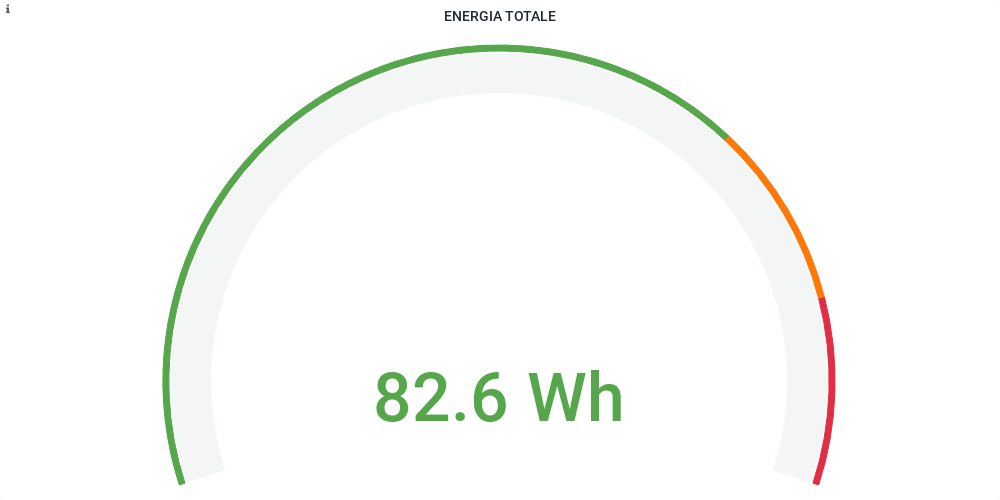
\includegraphics[width=0.5\textwidth]{image43}
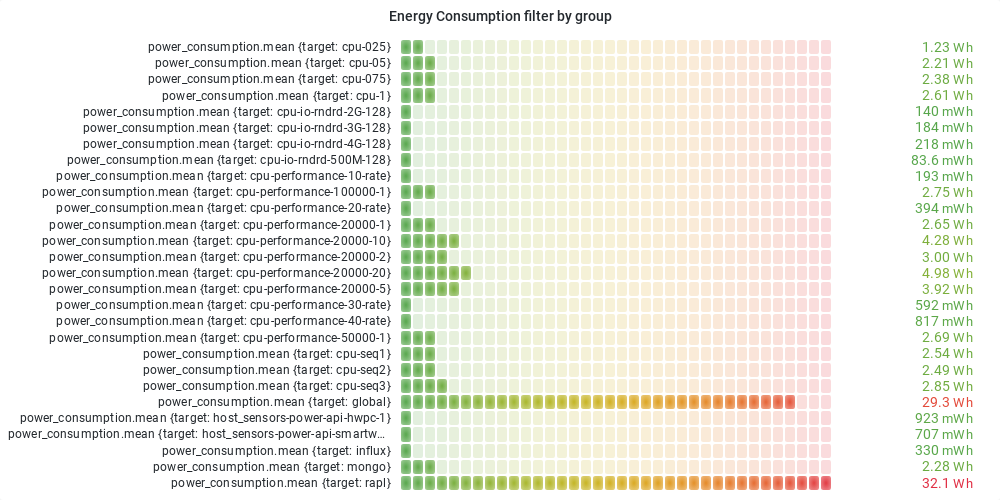
\includegraphics[scale=0.4]{image41}
{L'energia media consumata rientra negli standard delle CPU moderne.}
\end{figure}
\begin{figure}[h]
\caption{CONSUMI ENERGETICI DATABASE}
\centering
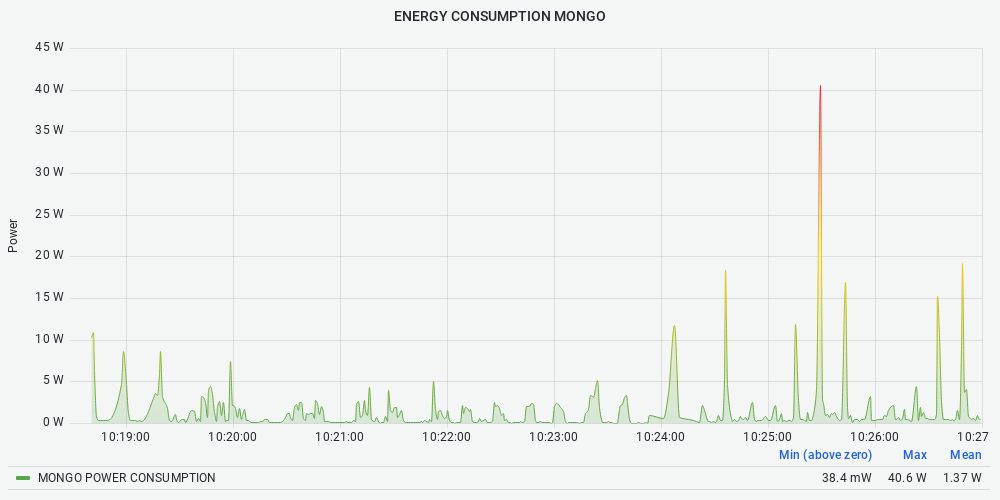
\includegraphics[scale=0.4]{image4}
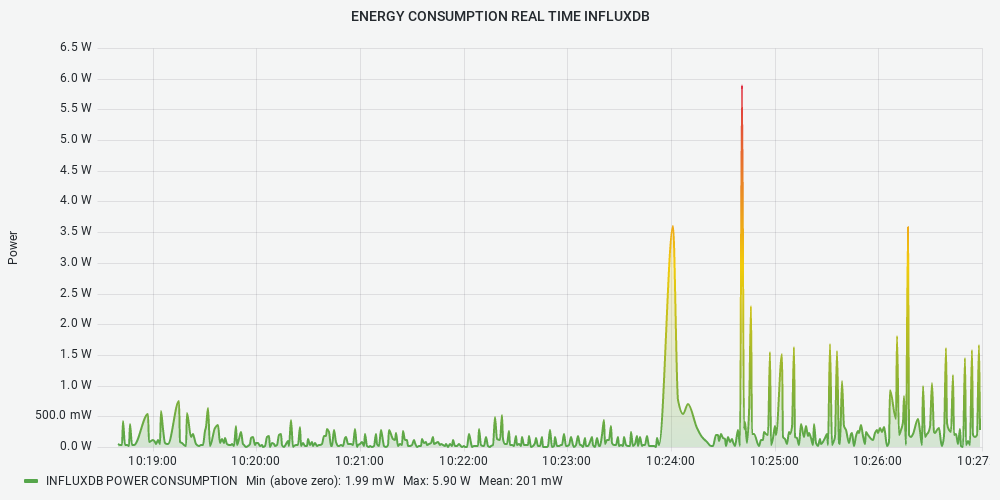
\includegraphics[scale=0.4]{image7}
\begin{flushleft}
{Vengono analizzati i consumi energetici dei database coinvolti nell'utilizzo di POWERAPI}
\end{flushleft}
\end{figure}

\begin{figure}[h]
\caption{SEQUENTIAL-CPU-TEST}
\centering
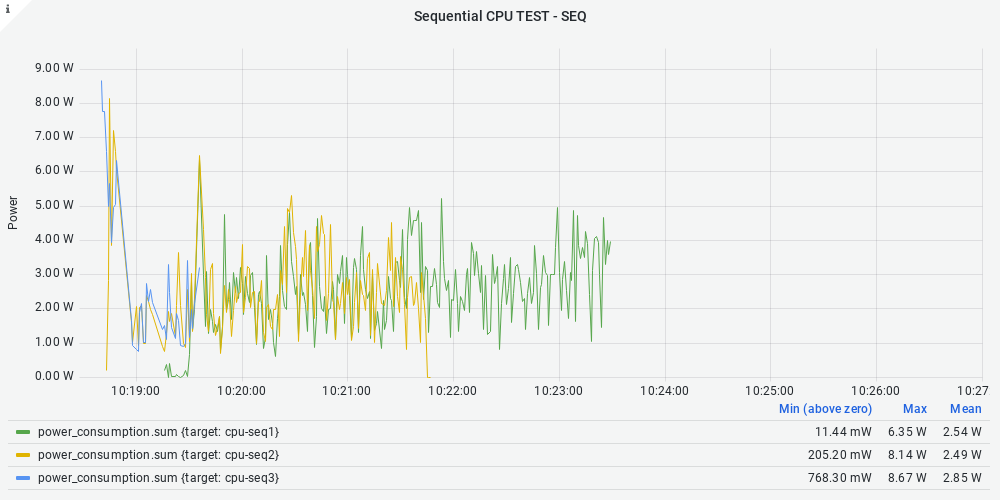
\includegraphics[scale=0.4]{image25}
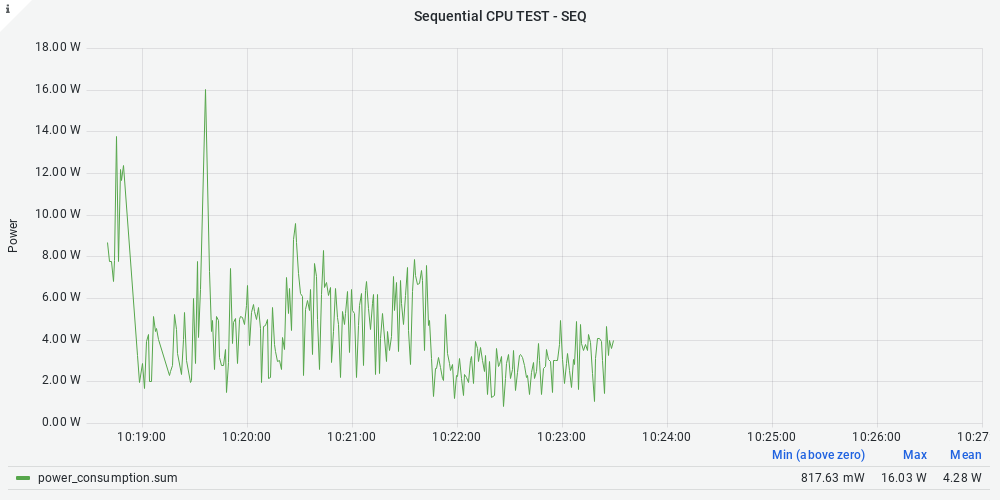
\includegraphics[scale=0.4]{image34}
\begin{flushleft}
Tre diverse run di sysbench cpu - rispettivamente con tre diverse tempistiche. Test base per verificare l'incremento dei consumi energetici all'incremento dei container docker in esecuzione.
\end{flushleft}
\end{figure}


\begin{figure}[h]
\caption{CPU-PERFORMANCE-N-RATE}
\centering
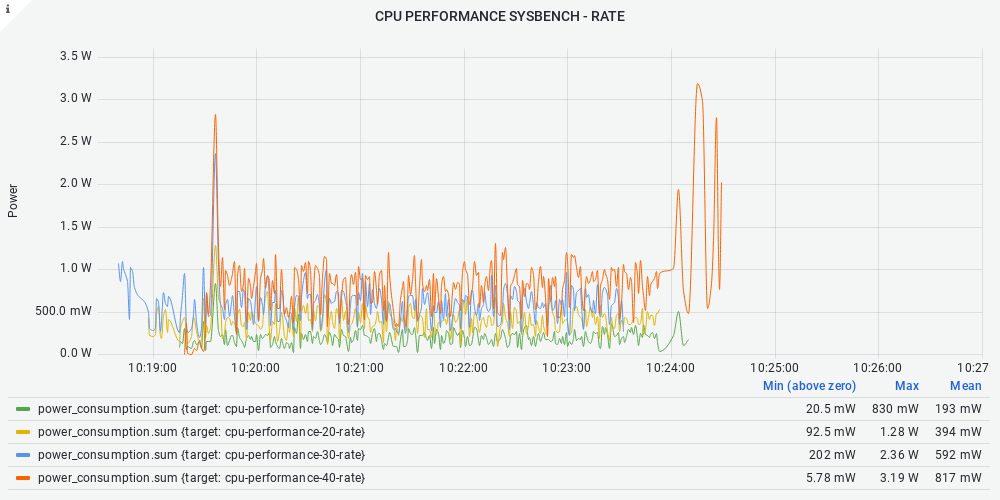
\includegraphics[scale=0.4]{image19}
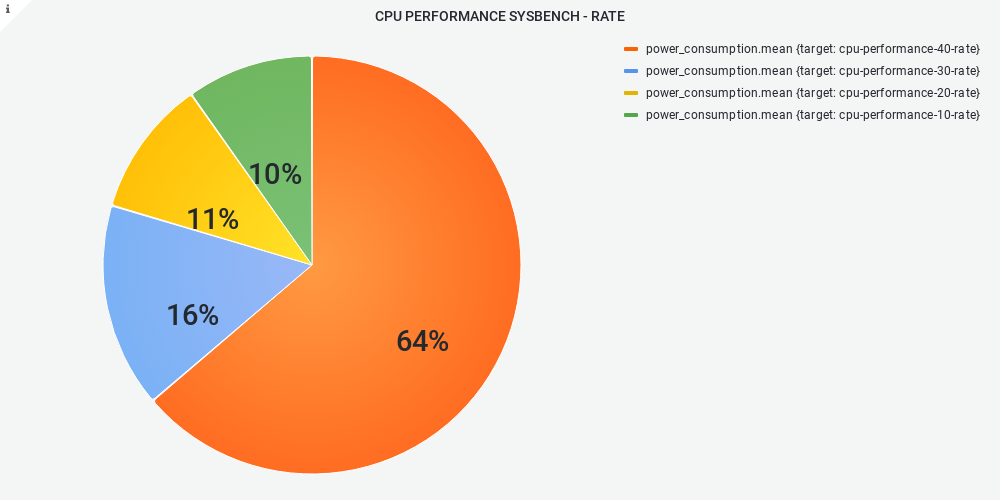
\includegraphics[scale=0.4]{image37}
\begin{flushleft}
Ogni container rappresenta una run sysbench variando il parametro rate.
\begin{center}
\textbf{N-rate : Tasso medio di transazioni.}
\\
\end{center}
Si vede come all'incrementare del tasso medio di transazioni (RATE) incrementano i consumi energetici.
\end{flushleft}
\end{figure}


\begin{figure}[h]
\caption{CPU-PERFORMANCE-P-N (threads)}
Il benchmark è configurato con il numero di thread simultanei e il numero massimo per verificare se è un numero primo.
\begin{flushleft}
\begin{itemize}
\item Ogni container rappresenta una run sysbench con questi parametri :
\begin{itemize}
\item P : cpu-max-prime
\item N : number of threads
\end{itemize}
\end{itemize}
Variando il numero di threads. 
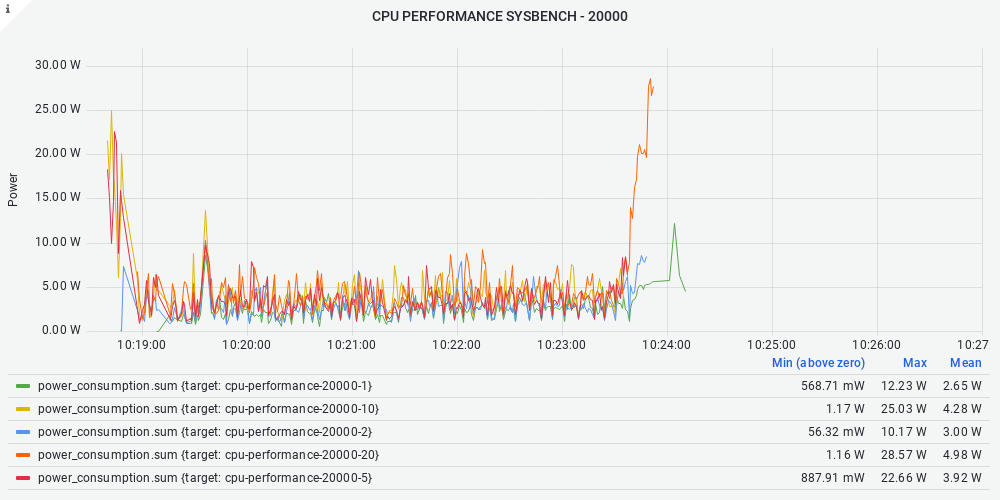
\includegraphics[scale=0.4]{image10}
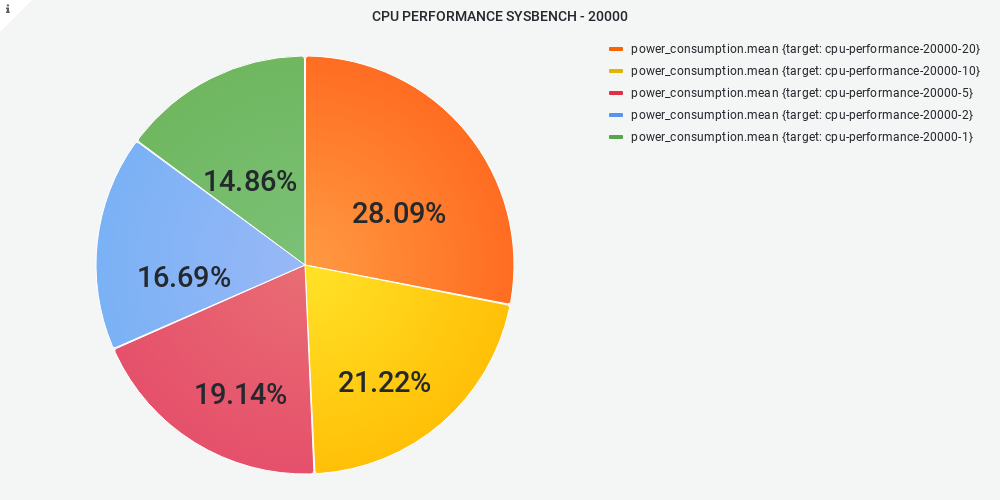
\includegraphics[scale=0.4]{image38}
\\ Si vede come all'incrementare del numero di threads coinvolti nel test, incrementano i consumi energetici.
\end{flushleft}
\end{figure}
\begin{figure}[h]
\caption{CPU-PERFORMANCE-P-N (cpu-max-prime)}
\begin{flushleft}
Variando cpu-max-prime.
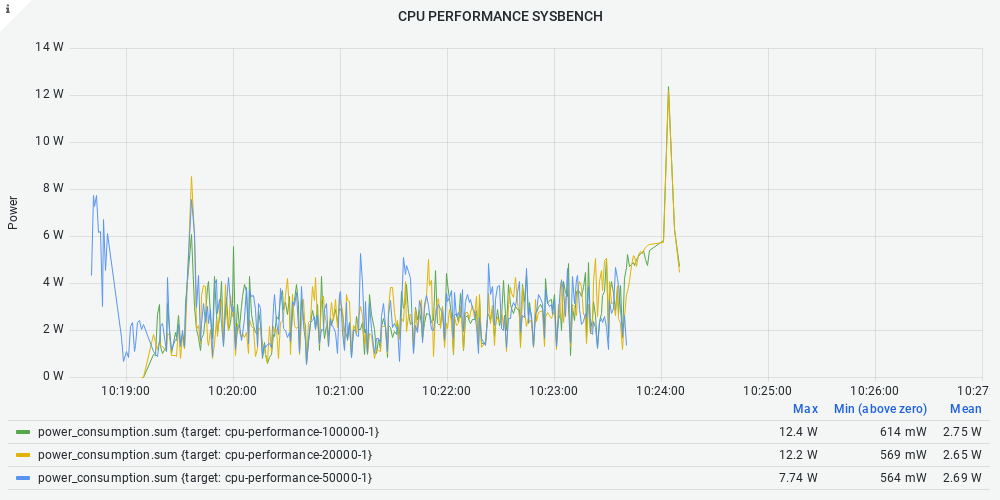
\includegraphics[scale=0.4]{image8}
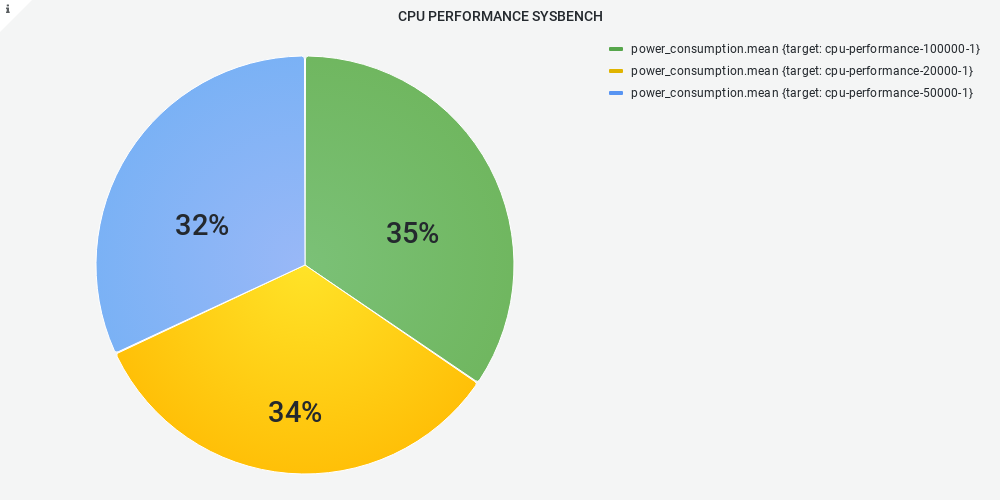
\includegraphics[scale=0.4]{image39}
\end{flushleft}
\end{figure}


\begin{figure}[h]

\caption{CPU-PERFORMANCE-N-RATE}
\centering
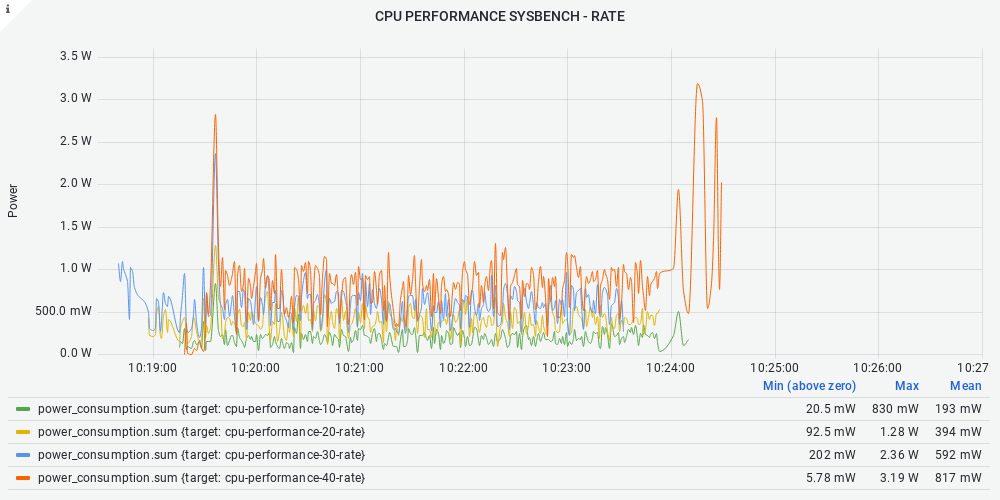
\includegraphics[scale=0.4]{image19}
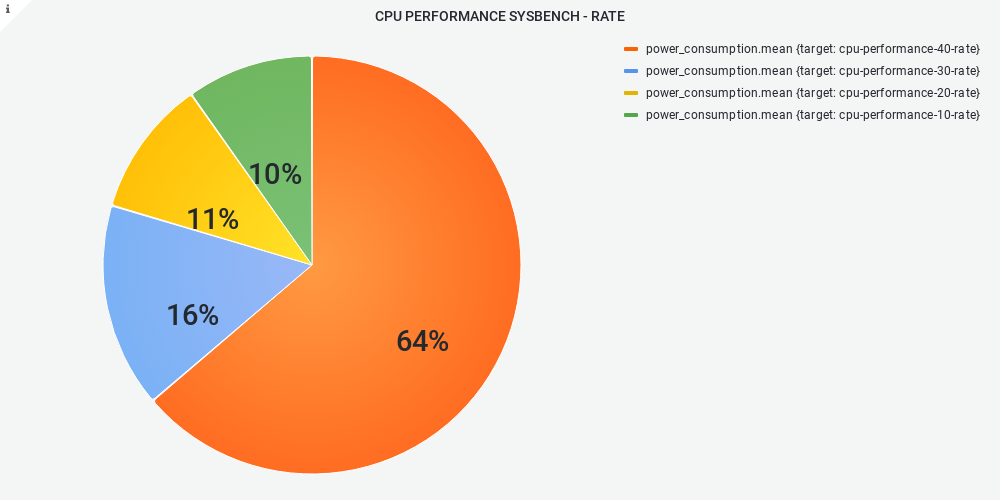
\includegraphics[scale=0.4]{image37}
\begin{flushleft}
Ogni container rappresenta una run sysbench variando il parametro rate.
\begin{center}
\textbf{N-rate : Tasso medio di transazioni.}
\\
\end{center}
Si vede come all'incrementare del tasso medio di transazioni (RATE) incrementano i consumi energetici.
\end{flushleft}
\end{figure}

\begin{figure}[h]
\caption{CPU-PERFORMANCE-CPUS-LIMIT}
\centering
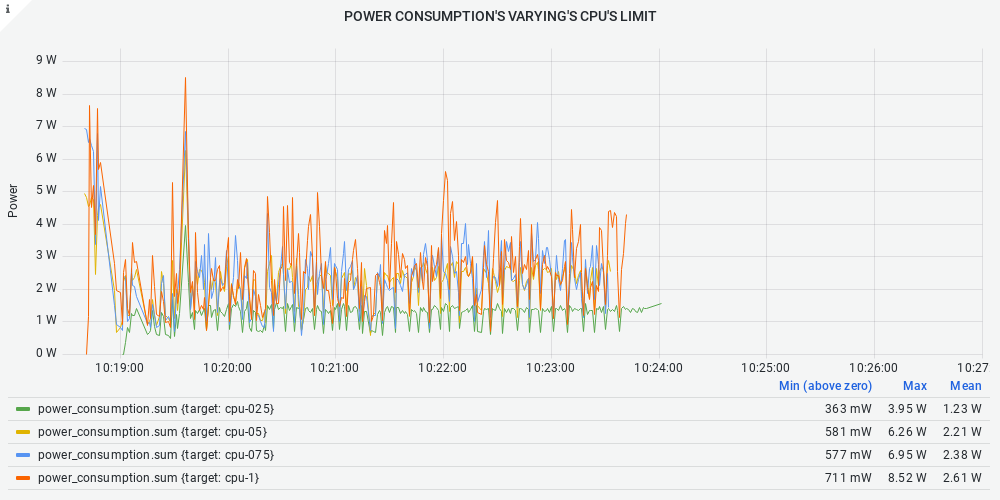
\includegraphics[scale=0.4]{image30}
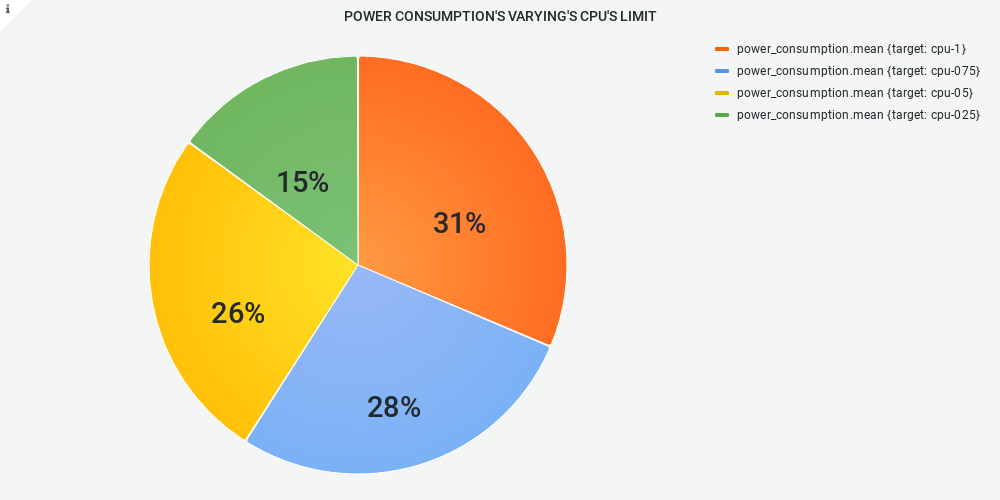
\includegraphics[scale=0.4]{image35}
\begin{flushleft}
In questi test viene usato il comando '--cpu=x' che permette di limitare l'utilizzo della cpu.
Si vede come all'incrementare della cpu assegnata incrementano i consumi energetici.
\end{flushleft}
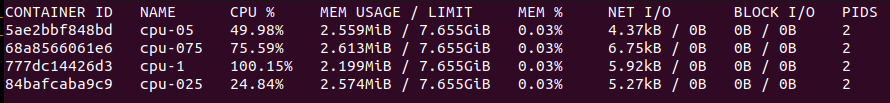
\includegraphics[scale=0.4]{cpus}
\begin{flushleft}
{La schermata permette di vedere la percentuale di CPU assegnata ad ogni container}
\end{flushleft}
\end{figure}

\begin{figure}[h]
\caption{CPU-IO-RNDRD-S-N}
\centering
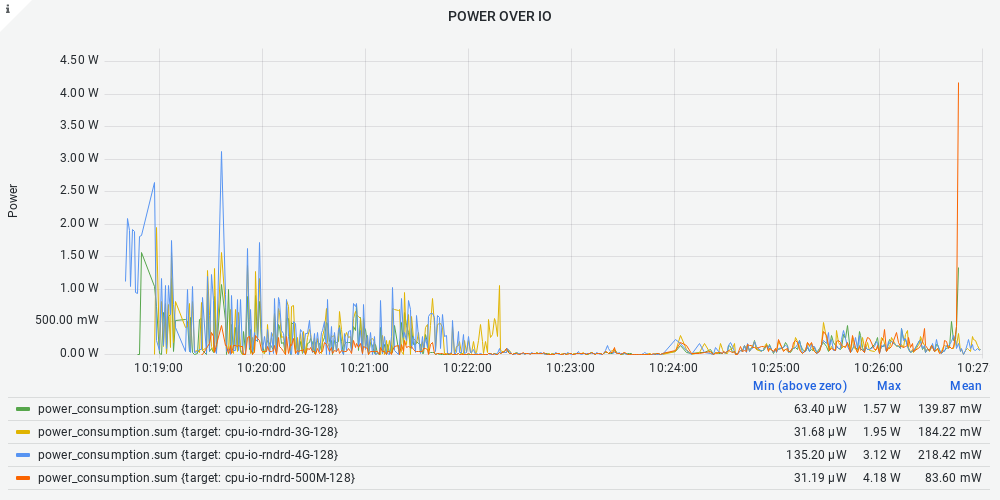
\includegraphics[scale=0.4]{image33}
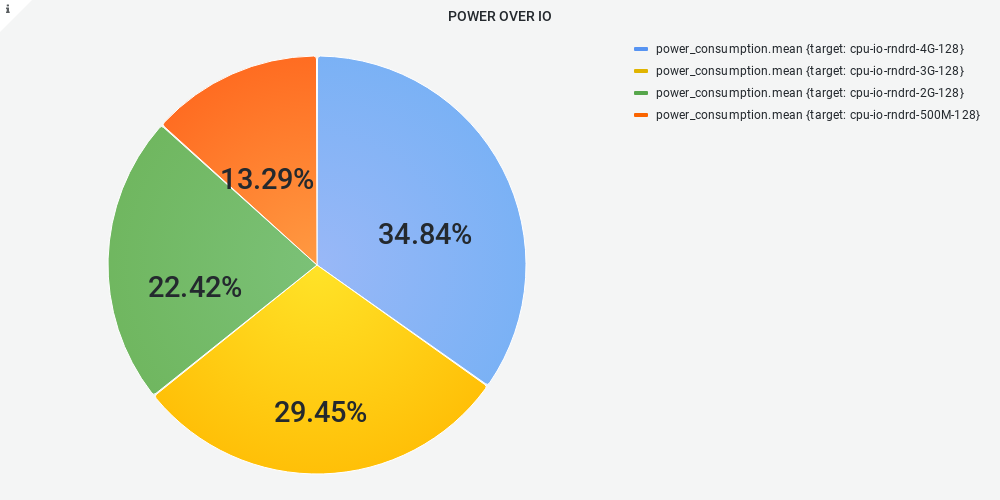
\includegraphics[scale=0.4]{image36}
\begin{flushleft}
In queste run viene testato sysbench IO.
\begin{itemize}
\item S: --file-total-size (grandezza di 1 file)
\item N: --file-num (numero di file)
\end{itemize}
\end{flushleft}
\begin{flushleft}
Si vede come all'incrementare della dimensione dei file, incrementano i consumi energetici.
\end{flushleft}
\end{figure}


\end{document}